\chapter{Introduction}

\section{Overview}
Pan-and-Tilt Unit (PTU) is a stabilised 2-axes platform mounted on the Idris electric vehicle that holds a panoramic camera. This vehicle is used for the research and drives over the curved surfaces \cite{ProjectIdris}. PTU has a built in functionality to stabilize at the chosen position: in case the rover drives up the hill camera will stay vertical. In order to achieve camera verticality stabilization command could only be invoked once, when the rover is standing on the flat surface. Its position could also be adjusted manually if it is on a curved surface and then stabilization command could be issued.

\section{Problem analysis}
To ensure stability of the camera PTU uses gyroscopes, which would be enough on its own in a perfect world. However, the well known problem of the gyroscopes is that their readings are affected by the different air temperature, magnetic effects, friction etc.\cite{HandbookOfModernSensors}. When PTU is issued with the stabilization command the platform slowly drifts on both axes and goes to the position which can be up to 20 degrees different from where it should be. This project will concentrate on fixing this particular issue as well as trying to enhance the overall system functionality. 

\section{Aim}
The aim of this project is to modify system which is currently in place and implement functionality to stabilize Pan-Tilt Unit with drift compensation. The system should be fully automated and perform drift rate calculation and following calibration on its own, when the appropriate request comes in from the client.

\section{Proposed Solution}
One of the possible solutions could be the use of the additional PTU functionality. It allows to cancel drift by specifying the calculated in advance drift rate in radians per second. The problem with this solution is that the drift rate can change if the surround environment changes (sun goes behind the clouds and air temperature drops affecting gyroscope readings). It is impossible to calculate new drift rate manually every 10 minutes.

The proposed solution is to automate the drift rate calculation so that it can be adjusted while driving. However this approach requires additional information about the current vehicle orientation in the space (its inclination angles with respect to gravity) to be able to predict required PTU position which will then be compared with the actual position and the drift rate that has been calculated. Electronic inclinometer can be used for this purpose. Inclinometer response is an electric signal representing an angle between the internal axis and the gravity vector \cite{HandbookOfModernSensors}. Accurate readings can only be obtained using the device if it is in a stable position and does not accelerate, otherwise it will provide erroneous data representing the sum of two vectors – earth gravity and acceleration. This imposes certain limitations. PTU drift rate calibration can only be performed when the vehicle does not move.

\section{Objectives}

The aims of this project are:
\begin{itemize}
\item To port current system from the Gumstix on to the Raspberry Pi.
\item To implement commands for the PTU stabilization and drift rate.
\item To develop drift rate calculation with following calibration.
\item To develop PTU verticality functionality.
\item To implement support for the new PTU functionality in the server side software.
\item To extend client side API to reflect new server functionality.
\end{itemize}

\section{Schedule and Project Management}
The length of the project is a bit less than 15 weeks. First week will be spent on the problem analysis, background research and Outline Project Specification production. In the middle of the project there will be poster production which should take few days and Easter break takes another week of the project time. Production of the final report, its review and proof reading will take another week. Essential it leaves us with a bit less that 12 weeks for system development.

Due to the tight time-frame imposed for the development of the system, an agile system development methodology will be followed. Agile development has a focus on generating working software prototypes quickly in cycles, rather than the classical approach of thorough documentation and following a strict plan. During software development there are likely to be unexpected technical difficulties that appear and need to be overcome, which can put the project behind the schedule.

The agile methodology attempts to provide the project with a clear direction by regularly assessing the development of the project at the end of each iteration, and interacting with the client to ensure the project is coming closer by fulfilling its requirements. When the progress of the project is assessed regularly, it gives the opportunity to steer it back into the right direction if there are evidences that the course development is moving away from the
target. The waterfall method which has a single fixed completion date at which the project completes and should be ready to deployed runs the risk of delays if the system does not come together as planned. If the project is abandoned at any point before it is completed there is unlikely to be even a partially working system completed. Thus the agile approach greatly reduces both development time and costs \cite{AgileManifesto}.

Following the initial evaluation of the different software development methodologies the feature-driven development methodology was chosen. At different stages of this project work will focus on the different parts of the system. In each such part there is a set of clearly identifiable features which are required for the final system to work. At the begging of the project consultation with the client (project supervisor) were conducted to identify overall model of the system. At the following meetings overall model was shaped and feature list build. The development of the system will be organised into iterations of relatively short 2 week cycles, with a set of working features produced at the end of each cycle.

Iteration 0 will focus on porting code to the new platform. It is not expected that system will work straight away, but after minor code adjustments it should have basic features working.

Iteration 1 has an aim of implementing new commands in the PTU TASS library.

Iteration 2 will focus on drift rate calculation algorithm development and testing. This iteration builds on the functionality laid town in the previous cycle and incorporates the ability to calculate drift rate. Following platform stabilization with the calculated drift rate. 

Iteration 3 will depend on the work done during all previous cycles. Without successful completion of all previous steps this iteration will not make any sense since there will be nothing to incorporate. In this iteration server side software will be updated to make use of the new features in the PTU TASS library. Client side API will be changed as well to reflect new functionality of the server.

At the end of which cycle, there will be a break and client consulted as to whether he feels that the project is continuing in the right direction.


The project schedule on the figure ~\ref{fig:ProjectSchedule} illustrates all the main tasks and planed deliverables.

\begin{landscape}
\begin{figure}[H] 
\centering
\centerline{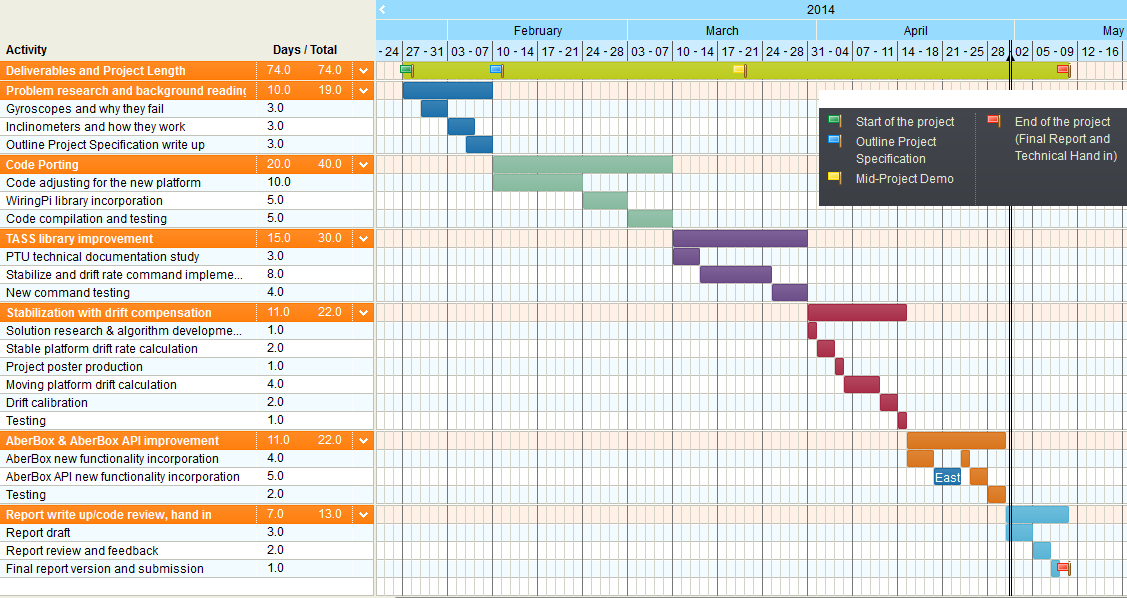
\includegraphics[scale=0.8]{./images/ProjectSchedule}}
\caption{Project schedule}
\label{fig:ProjectSchedule}
\end{figure}
\end{landscape}